	\documentclass[11pt,a4paper]{article}
\usepackage{geometry}
\usepackage{amsmath}
\usepackage{amssymb}
\usepackage[utf8]{inputenc}  
\usepackage[T1]{fontenc}  
\usepackage{enumitem}
\usepackage{sectsty}
\usepackage{xcolor}
\usepackage{graphicx}
\usepackage{french}
\usepackage{float} 
\usepackage{listings}
 




%%%%%%%%%%%%%%%%%%
%% MISE EN PAGE %%
%%%%%%%%%%%%%%%%%%
% Marges
\geometry{hmargin=2.5cm,vmargin=2cm}

% On définit les deux couleurs utilisées
\definecolor{couleur_section}{RGB}{0,86,108}
\definecolor{couleur_subsection}{RGB}{4,110,129}

% On personnalise chacun des titres à l'aide des commandes "sectionfont", "subsectionfont", etc.
\sectionfont{\color{couleur_section} \scshape}
\subsectionfont{\color{couleur_subsection}}
\subsubsectionfont{\itshape}

% Mise en forme des listing Python
\definecolor{codegreen}{rgb}{0,0.6,0}
\definecolor{codegray}{rgb}{0.5,0.5,0.5}
\definecolor{codepurple}{rgb}{0.58,0,0.82}
\definecolor{backcolour}{rgb}{0.95,0.95,0.92}
 
\lstdefinestyle{mystyle}{
    backgroundcolor=\color{backcolour},   
    commentstyle=\color{codegreen},
    keywordstyle=\color{magenta},
    numberstyle=\tiny\color{codegray},
    stringstyle=\color{codepurple},
    basicstyle=\ttfamily\footnotesize,
    breakatwhitespace=false,         
    breaklines=true,                 
    captionpos=b,                    
    keepspaces=true,                 
    numbers=left,                    
    numbersep=5pt,                  
    showspaces=false,                
    showstringspaces=false,
    showtabs=false,                  
    tabsize=2
}
 
\lstset{style=mystyle}


\begin{document}

    %%%%%%%%%%%%%%%%%%%
    %% PAGE DE GARDE %%
    %%%%%%%%%%%%%%%%%%%
    \begin{titlepage}
        \centering
        
\includegraphics[width=0.40\textwidth]{uca.png}\par\vspace{1cm}
        {\scshape\LARGE Université Clermont Auvergne \par}
        {\scshape École Universitaire de Physique et d'Ingénierie \par}
        \vspace{2cm}
        \noindent\rule{\textwidth}{0.5pt}\par
        {\scshape\Large Etude d'un article scientifique de \textbf{Deep Learning}\par}
        \vspace{0.5cm}
        {\huge\bfseries Context encoder\par}
        \noindent\rule{\textwidth}{0.5pt}\par
        \vspace{5cm}
        {\Large\itshape Lucas TOURON\par}
        {\Large\itshape Sagaf YOUSSOUF\par}

        \vfill

        % Bottom of the page
        {\large 2019 - 2020\par}
    \end{titlepage}



    %%%%%%%%%%%%%%%%%%%%%%%%
    %% TABLE DES MATIERES %%
    %%%%%%%%%%%%%%%%%%%%%%%%
    \tableofcontents
    \newpage
    
    
    
    %%%%%%%%%%%%%%%%%%%%%%%%
    %% CONTENU DU RAPPORT %%
    %%%%%%%%%%%%%%%%%%%%%%%%
    \section{Résumé de l'article}
    Le \textbf{Context-Encoder}, par analogie aux auto-encodeurs, est une méthode d'apprentissage non supervisée permettant de faire de l'\textbf{inpainting}. L'\textbf{inpainting} est une technique permettant de reconstruire des régions manquantes dans une image. \\
    Le context-encoder est étroitement lié aux \textbf{auto-encodeurs} puisqu’il partage une architecture similaire d’un encodeur et d’un decodeur. Comme on l’a vu en TP, les auto-encodeurs sont des types de réseaux neurones qui nécessitent des exemples de données mais pas (ou peu) d’annotations. Dans sa version la plus simple, ce type de réseaux de neurones apprend à l’aide de la descente de gradient.\\
    L'encodeur est constitué d'un réseau de type CNN.
    Le context-encodeur prend en compte un maximum de \textbf{caractéristiques} de l'image existante. Il est entrainé à l'aide de la méthode de \textbf{réseaux adverses génératifs}.\\
    La fonction objectif est déterminée de 2 manières différentes : par reconstruction et par GAN. Il est aussi possible de fusionner ces deux méthodes, ce qui s'avère être la méthode la plus aboutie selon plusieurs tests effectués sur différentes bases d'images.\\
    
    
    \section{Description de la 	méthode proposée}
    Nous avons définit les \emph{concext-encodeur} comme étant des réseaux de neurones convolutifs (CNN) qui prédisent les parties manquantes d’une scène à partir des régions voisines de l’image. L’architecture globale de cette méthode est composée d’un pipeline encodeur/decodeur avec une couche entièrement connectée qui fait office de canal entre l’encodeur et le decodeur. Le réseau est entraîné de manière non supervisé. Pour réussir cette tâche, les auteurs ont démontré que le réseau doit être en mesure de comprendre le contenu de l’image. Pour cela, le context-encoder est entraîné conjointement avec une fonction perte appelée \emph{« reconstruction loss »}  et une autre fonction appelée \emph{« adversial loss »}.

    \subsection{Le pipeline encodeur-decodeur}
        Le pipeline prend une image en entrée avec des régions manquantes de taille $227*227$ et produit une représentation caractéristique de cette image. L’encodeur peut être substitué par n’importe quel architecture réseau comme AlexNet.\\
    La forme des régions manquantes peut varier : un carré au centre de l’image, plusieurs carrés ou encore des formes quelconques.\\
    A la suite, le decodeur prend cette représentation et produit le contenu de l’image manquante. Le decodeur est une suite de couche \emph{UpConv/deconv/frac-strided-conv}. L’encodeur et le decodeur sont liés par un canal de couche \textbf{fully connected}.
        \begin{figure}[H]
            \centering
            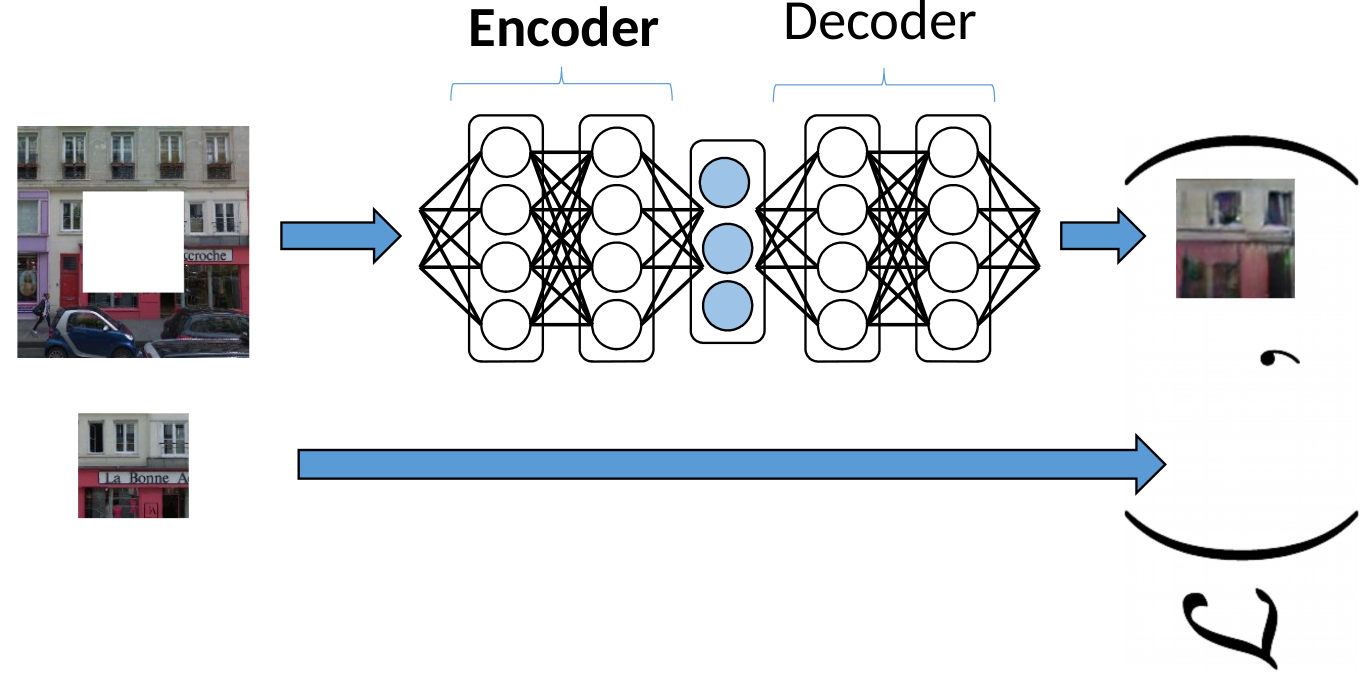
\includegraphics[scale=0.2]{pipeline.png} 
            \caption{Pipeline encodeur-decodeur}
        \end{figure}
        
        \begin{figure}[H]
            \centering
            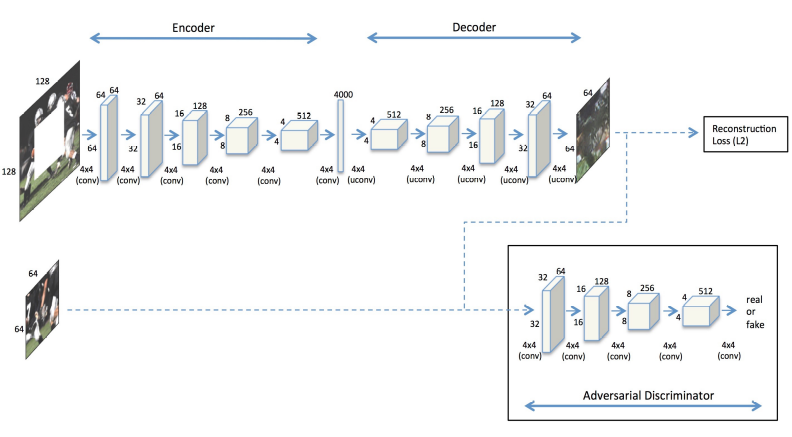
\includegraphics[scale=0.55]{architecture.png} 
            \caption{Architecture du context encodeur}
        \end{figure}

        \subsection{L'encodeur}
            L’encodeur utilisé est dérivé de l’architecture d’AlexNet. Il prend une image d’entrée de taille $227*227$. Les 5 premières couches de convolution et les couches de pooling suivantes sont utilisées pour calculer une représentation abstraite de caractéristiques \emph{(de dimensions $6*6*256$)}. Puisque l’architecture de l’encodeur est limité à des couches de convolutions, il n’y a aucun moyen de propager les informations à travers les cartes caractéristiques. C’est pour cette raison que l’architecture utilise une couche \emph{fully connected} ou \emph{inner product}. Contrairement aux auto-encodeurs, l’architecture n’essaie pas de reconstruire l’image entière. Les dimensions du latent feature sont donc de $6*6*256=9216$ pour l’encodeur et le decodeur. En utilisant une couche entièrement connectée, le nombre de paramètres va considérablement augmenter (\textbf{$> 100M$ !}). L’entraînement sera donc très complexe.  Pour y remédier, on utilise une couche \textbf{channel-wise fully connected} décris ci-dessous. 
        
        \subsection{La couche \emph{channel-wise fully connected}}
            Contrairement à une couche entièrement connectée, cette couche n’a pas de paramètres reliant les cartes d’activations. Elle va juste propager l’information à l’intérieur des activations pour chaque carte de caractéristiques.  Le nombre de paramètre de cette couche est $m*n$ \emph{(en ignorant les biais)} alors qu'une couche de entièrement connectée dont le nombre de paramètre est de $m*n^4$.

        \subsection{Le decodeur}
            La deuxième partie du pipeline est le decodeur. Il génère les pixels de l’image à l’aide des fonctions de l’encodeur.\\
            Comme on l’a déjà précisé, les caractéristiques de l’encodeur et du decodeur sont reliés ensemble à l’aide de la couche \emph{channel-wise fully connected}. Cette couche est suivi d’une série de 5 couches ascendants \emph{(up-convolutional)} avec des filtres appris et des fonctions d’activation ReLU. 
            
        \subsection{Le fonction perte}
            Pour entraîner le context-encodeur, on fait une régression au contenu de vérité de terrain de la région manquante de l’image.  Il existe plusieurs façons d’estimer une région d’images manquantes compatible avec le concept de context-encodeur. Les auteurs de cet article ont modélisé ce comportement avec une fonction de perte découplée.  Trois types de fonctions de perte ont été étudié :
            \begin{enumerate}[noitemsep]
                \item \textbf{La perte de reconstruction (reconstruction loss L2)}\\
                Cette fonction perte assure la capture de la structure globale de la région manquante et de la cohérence par rapport à son contexte. Cette fonction perte renvoie une image flou. C'est pour cette raison que les auteurs on fait appel a une fonction perte basée sur le GAN.
                \item \textbf{L’adversial loss}\\
                L’adversial loss quand à lui tente de faire paraître la prédiction réelle en choisissant un mode particulier dans la distribution. Elle est basés sur les réseaux adverses génératifs (GAN). Il s’agit d’une classe d’algorithme d’apprentissage non-supervisé permettant de générer des images avec une forte degré de réalisme. Cette méthode a été adapté en modélisant le générateur du GAN par le context-encodeur. L’approche exploitée dans l’article consiste à conditionner uniquement le générateur et non le discriminateur. L'adversial loss est utilisée dans l'optique d'être combiné avec la reconstruction loss. Cette méthode renvoie une région d'image incohérente mais qui s'avérera utile en la combinant avec la region flou obtenu par le loss L2.
                \item \textbf{Le joint loss}\\
                Cette fonction perte est la combinaison des deux méthodes présentées ci-dessus. On peut la représenter sous forme mathématique, comme suit :
                \begin{figure}[H]
                    \centering
                    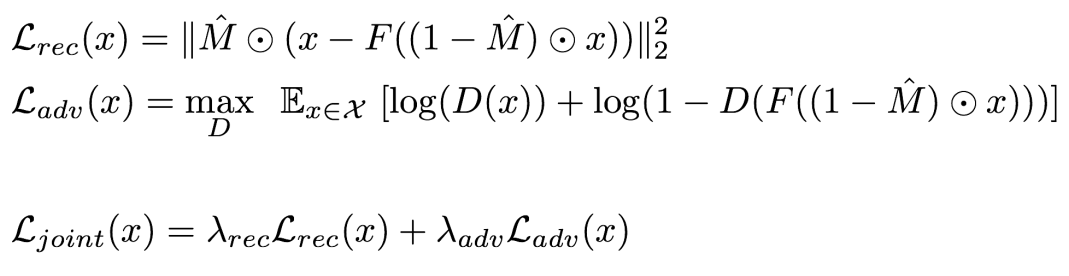
\includegraphics[scale=0.34]{formule.png} 
                    \caption{Forme mathématique des fonctions perte}
                \end{figure}
                Où :
        		\begin{itemize}[noitemsep]
			        \item $M$ est un masque binaire de même taille que l'image. Il vaut $1$ pour les régions manquantes et $0$ dans le cas contraire.
			        \item $F$ est l'image de sortie du context encoder.
			        \item $\odot$ correspond à un produit matriciel de Hadamard \emph{(une multiplication terme à terme)}.
			        \item $D$ est le modèle du discriminateur.
		        \end{itemize}
                Une fois combiné avec la méthode par perte de reconstruction, on obtient un très bon résultat.\\
            \end{enumerate}

            Voici une illustration des résultats des différentes fonctions de perte :
            \begin{figure}[H]
                \centering
                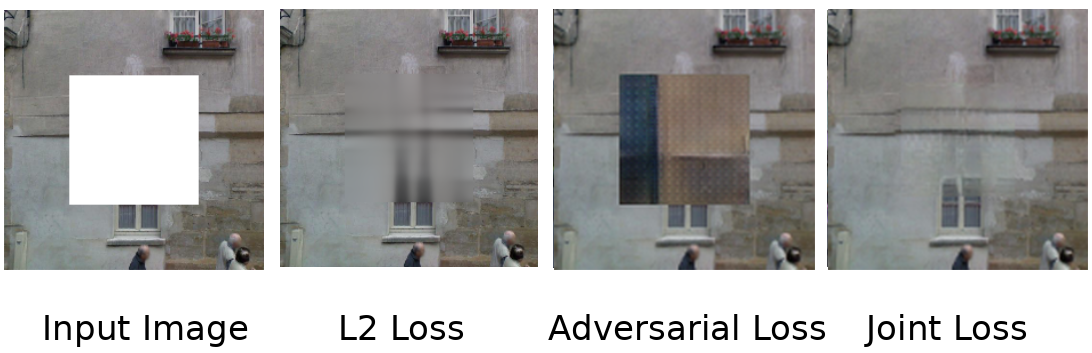
\includegraphics[scale=0.35]{loss.png} 
                \caption{Illustration des résultats des fonctions de perte}
            \end{figure}
            
    \section{Description des tests}
        \subsection{Détails de l'implémentation}
            Le code original de l’article (\emph{(cf ref 2)} est implémenté en \texttt{Torch}. Nous avons également essayé de tester cette implémentation sur un GPU Nvidia Jetson TX2 (utilisé pour les cours de GPU). Cependant, nous n'avons pas pu aboutir à un résultat en raison d'incompatibilités avec CUDA 10.\\
            Pour des fins de simplicité et pour faire le lien avec les cours de Deep Learning, on a utilisé une implémentation codée en \texttt{Python} avec \texttt{Keras}. Elle est disponible sur Github \emph{(cf ref 3)}. L'objectif des tests est d’expérimenter les capacités et les limites du context-encodeur.
        \subsection{L'encodeur}
        
L'étape de convolution du modèle de l'encodeur est décomposée ainsi :\\
Une couche de 32 convolutions de taille $3*3$, qui prend en entrée la taille de l'image d'entrée \emph{($32*32$)}, avec un pas de balayage de 2 dans chaque direction et sans padding. Cette couche de convolution est suivie d'une couche d'activation utilisant la fonction d'activation \texttt{LeakyRELU} pour introduire des complexités non-linéaires au modèle.\\
Ensuite, on fait appel à une couche de normalisation de batch, qui sert à optimiser les performances du réseau en normalisant les poids des activations. Cette couche est suivie d'un jeu de couche de normalisation de batch, de trois couches de convolutions \emph{(de taille 64, 128 et 512)} et des couches d'activations \texttt{LeakyRELU}.               
            \begin{lstlisting}[language=Python, caption=Code Python de l'encodeur]
# encodeur
model.add(Conv2D(32, kernel_size=3, strides=2, input_shape=self.img_shape, https://www.xm1math.net/doculatex/listes.htmlpadding="same"))
model.add(LeakyReLU(alpha=0.2))
model.add(BatchNormalization(momentum=0.8))
model.add(Conv2D(64, kernel_size=3, strides=2, padding="same"))
model.add(LeakyReLU(alpha=0.2))
model.add(BatchNormalization(momentum=0.8))
model.add(Conv2D(128, kernel_size=3, strides=2, padding="same"))
model.add(LeakyReLU(alpha=0.2))
model.add(BatchNormalization(momentum=0.8))
model.add(Conv2D(512, kernel_size=1, strides=2, padding="same"))
model.add(LeakyReLU(alpha=0.2))
model.add(Dropout(0.5)) \end{lstlisting}
        
        \subsection{Le decodeur}
            Le décodeur est composé d'une suite respective de 3 couches comme suit :
		    \begin{itemize}[noitemsep]
	            \item Une couche d'UpSampling 2D
	            \item Une couche d'activation (de type \texttt{relu} et \texttt{tanh})
	            \item Une couche de normalisation de batch
            \end{itemize}
La couche d'UpSampling est une couche simple, sans poids, qui permet de doubler les dimensions d'entrée lorsqu'elle est suivie d'une couche de convolution.            
            \begin{lstlisting}[language=Python, caption=Code Python du decodeur]
# decodeur
model.add(UpSampling2D())
model.add(Conv2D(128, kernel_size=3, padding="same"))
model.add(Activation('relu'))
model.add(BatchNormalization(momentum=0.8))
model.add(UpSampling2D())
model.add(Conv2D(64, kernel_size=3, padding="same"))
model.add(Activation('relu'))
model.add(BatchNormalization(momentum=0.8))
model.add(Conv2D(self.channels, kernel_size=3, padding="same"))
model.add(Activation('tanh'))\end{lstlisting}

        \subsection{Le discriminateur du GAN}
            Le discriminateur est composé d'une suite respective de 3 couches comme suit :
		    \begin{itemize}[noitemsep]
	            \item Une couche de convolution 2D
	            \item Une couche d'activation de type \texttt{LeakyReLU}
	            \item Une couche de normalisation de batch
            \end{itemize}
            Ensuite, il y a une couche qui transforme les données 2D en données 1D, pour ensuite les connecter à la couche dense de sortie.
            \begin{lstlisting}[language=Python, caption=Code Python du discriminateur]
# Discriminateur
model.add(Conv2D(64, kernel_size=3, strides=2, input_shape=self.missing_shape, padding="same"))
model.add(LeakyReLU(alpha=0.2))
model.add(BatchNormalization(momentum=0.8))
model.add(Conv2D(128, kernel_size=3, strides=2, padding="same"))
model.add(LeakyReLU(alpha=0.2))
model.add(BatchNormalization(momentum=0.8))
model.add(Conv2D(256, kernel_size=3, padding="same"))
model.add(LeakyReLU(alpha=0.2))
model.add(BatchNormalization(momentum=0.8))
model.add(Flatten())
model.add(Dense(1, activation='sigmoid'))
model.summary()\end{lstlisting}

        \subsection{Etapes de l'implémentation}  
        En premier lieu, on crée et on \texttt{compile} un modèle du discriminateur crée préalablement, en faisant appel à la fonction correspondante. La fonction perte utilisée est de type \texttt{binary-crossentropy} et l’\texttt{optimizer} utilisé est \texttt{Adam} avec un learning rate de $0.999$.\\ 
        On construit par la suite le générateur composé de l’encodeur et du décodeur. Ce générateur prend une image de bruit en entrée et génère l'image avec les régions manquantes. \\
        L’entraînement se fait seulement avec le générateur pour le modèle qui va combiner à la fois le discriminateur et le générateur. Le discriminateur prend en entrée l'image de sortie du générateur et détermine si elle est réelle ou pas .\\
        Enfin, nous créons un modèle constitué d'une combinaison des images générées par le générateur et par le discriminateur.\\
        Les résultats obtenus avec cette méthode sont illustrés dans la figure ci-dessous :
        \begin{figure}[H]
            \centering
            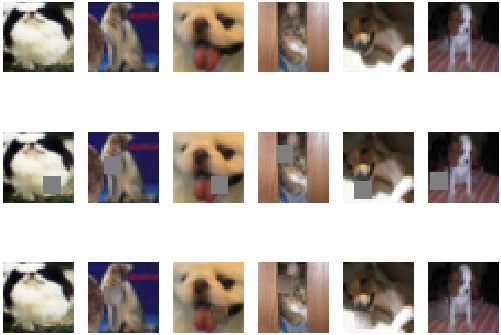
\includegraphics[scale=0.35]{resultat.png} 
            \caption{Exemples d'images reconstituées par le context encoder}
        \end{figure}
        En choisissant un nombre d'epoch de $3000$ et un batchsize de $64$, nous obtenons un bon résultat (accuracy de $99\%$), comme nous pouvons le voir dans la figure ci-dessous :
        \begin{figure}[H]
            \centering
            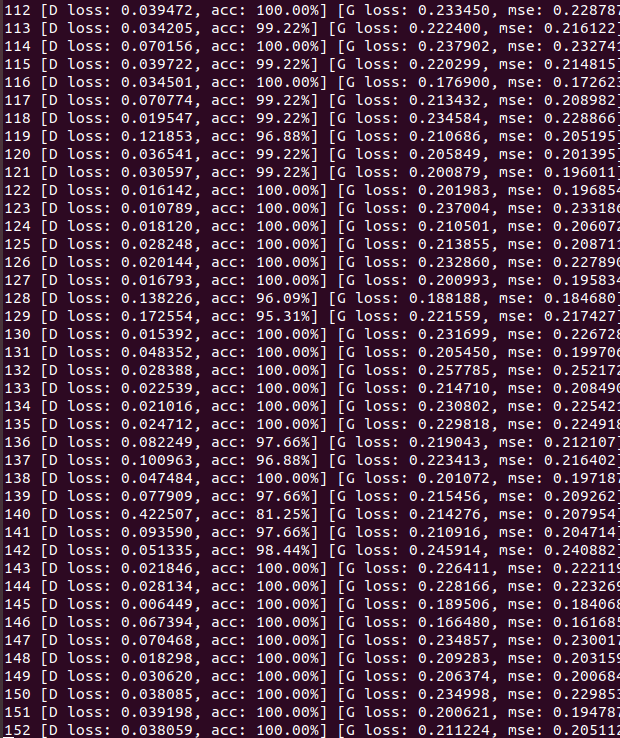
\includegraphics[scale=0.35]{result_performance.png} 
            \caption{Traces de sortie du context encoder}
        \end{figure}
    \begin{lstlisting}[language=Python, caption=Code Python de l'entrainement]
optimizer = Adam(0.0002, 0.5)

self.discriminator = self.build_discriminator()
self.discriminator.compile(loss='binary_crossentropy',
optimizer=optimizer,
metrics=['accuracy'])

self.generator = self.build_generator()

masked_img = Input(shape=self.img_shape)
gen_missing = self.generator(masked_img)

self.discriminator.trainable = False

valid = self.discriminator(gen_missing)

self.combined = Model(masked_img , [gen_missing, valid])
self.combined.compile(loss=['mse', 'binary_crossentropy'],
loss_weights=[0.999, 0.001],
optimizer=optimizer)\end{lstlisting}
    \section{Conclusion}
    Nous avons étudié un article scientifique présentant le contexte encoder. Nous avons démontré que les contexte-encoder sont des types de CNN permettant de générer des régions manquantes dans une image. Son architecture globale est composée d’un encodeur et d’un décodeur. Pour que les régions reconstruites soient plus réaliste, un modèle de réseaux de neurone de type GAN a été ajouté.\\ 
    L’étude de cet article nous a permis de mettre en exergue le concept des CNN appris en classe. Nous avons par exemple pu voir un cas d'utilisation d'un GAN dans des conditions réelles.

    %%%%%%%%%%%%%%%%%%%%%%%
    %% TABLE DES FIGURES %%
    %%%%%%%%%%%%%%%%%%%%%%%
    \newpage
    \listoffigures
    \newpage



    %%%%%%%%%%%%%%%%%%
    %% BIBLIOGRAPHY %%
    %%%%%%%%%%%%%%%%%%
    \begin{thebibliography}{9}
        \bibitem{contextencodeur} 
            Deepak Pathak, Phillip Krähenbühl, Jeff Donahue, Trevor Darrell, Alexei A. Efros\\
            \textit{Context encodeurs: Feature Learning by Inpainting}.\\
            UC Berkeley, CVPR, 2016.
            \\\texttt{https://people.eecs.berkeley.edu/\~{}pathak/context\_encodeur}
        \bibitem{github Pathak} 
            Deepak Pathak\\
            \textit{Github de Pathak}.
            \\\texttt{https://github.com/pathak22/context-encodeur}
        \bibitem{github Erik Linder Noren} 
            Erik Linder Noren\\
            \textit{Github de Erik Linder Noren}.
            \\\texttt{https://github.com/eriklindernoren/Keras-GAN/tree/master/context\_encodeur}
    \end{thebibliography}


\end{document}

